\documentclass{article}

\usepackage{graphicx}
\usepackage{tikz}
\usepackage{tikzsymbols}
\usetikzlibrary{calc,patterns,shapes.geometric}
\pagestyle{empty}
\usepackage[margin=0pt]{geometry}
\geometry{papersize={14in,12in}}

\def\centerarc[#1](#2)(#3:#4:#5){\draw[#1] ($(#2)+({#5*cos(#3)},{#5*sin(#3)})$) arc (#3:#4:#5);}

\begin{document}
	\begin{figure}
		\centering
		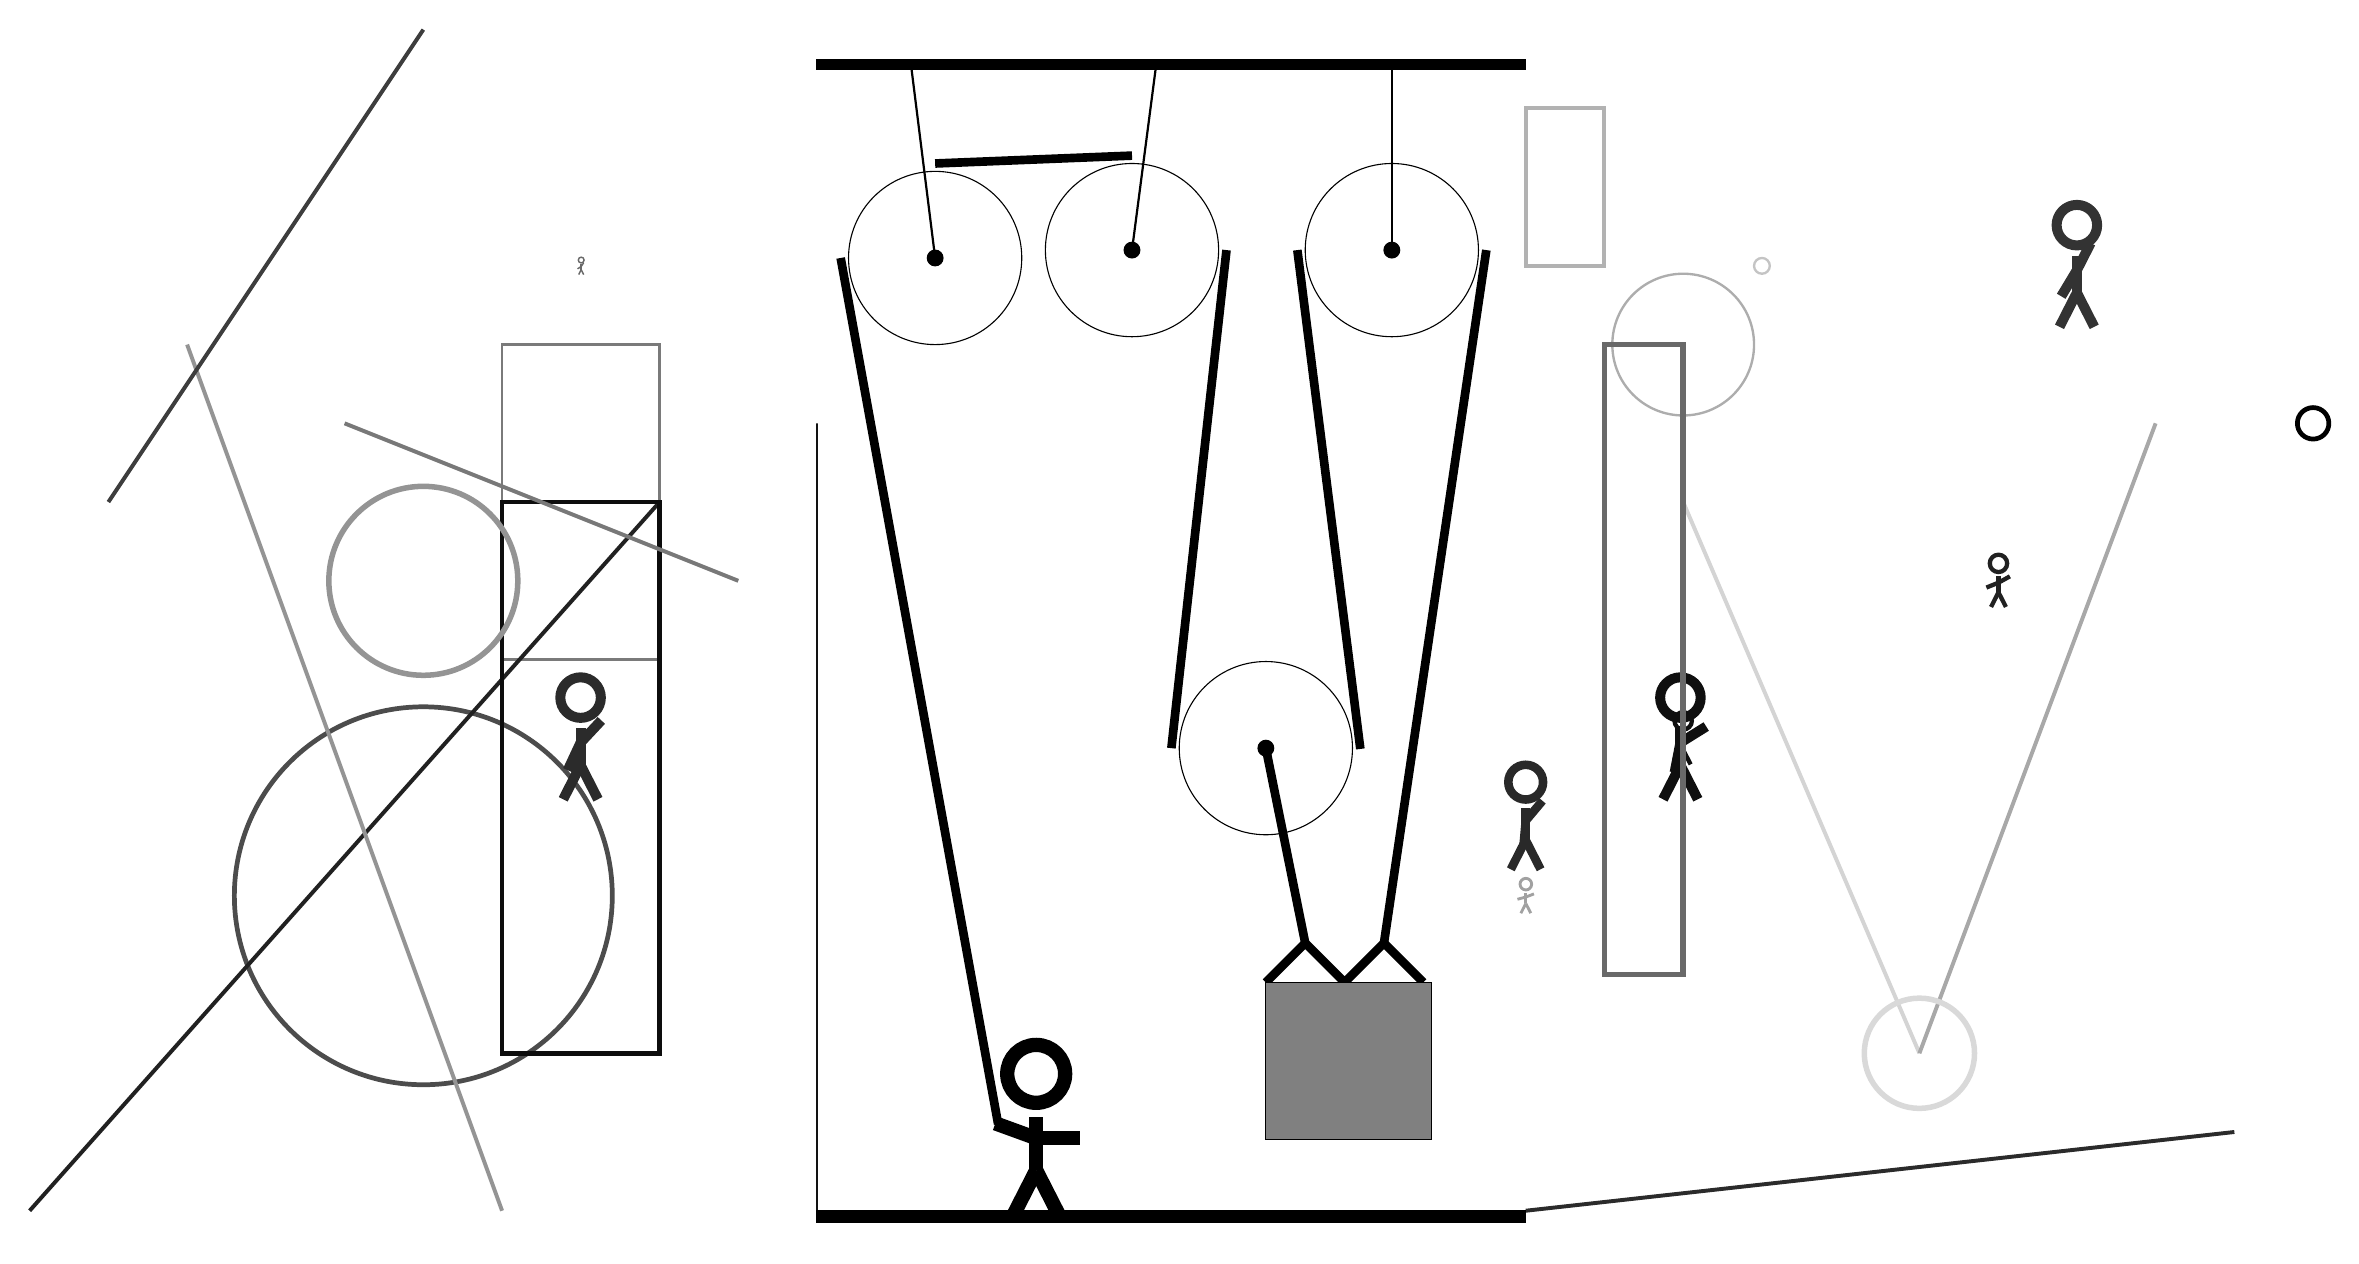
\begin{tikzpicture}
			%%%%% START %%%%%
			
			\draw[fill=black] (-3, 11.5) rectangle (6, 11.625);
			
			\draw (1, 9.2) circle (1.1);
			\draw[fill=black] (1, 9.2) circle (0.1);
			\draw[thick] (1, 9.2) -- (1.3, 11.5);
			
			\draw (4.3, 9.2) circle (1.1);
			\draw[fill=black] (4.3, 9.2) circle (0.1);
			\draw[thick] (4.3, 9.2) -- (4.3, 11.5);
			
			\draw (2.7, 2.875) circle (1.1);
			\draw[fill=black] (2.7, 2.875) circle (0.1);
			
			\node[line width=0.4mm, color=black!84] at (6, 2) {\Strichmaxerl[6][85][50]};
			
			\draw [line width=0.6mm, color=black!100](16, 7) circle (0.2);
			\draw [line width=0.6mm, color=black!70](-8, 1) circle (2.4);
			\node[line width=0.5mm, color=black!37] at (6, 1) {\Strichmaxerl[2][15][21]};
			\node[line width=0.3mm, color=black!80] at (13, 9) {\Strichmaxerl[7][59][63]};
			\draw[line width=0.5mm, color=black!17](8, 6) -- (11, -1);
			
			\draw[line width=0.3mm, color=black!93] (-3, 7) rectangle (-3, -3);
			\draw[line width=0.3mm, color=black!52] (-5, 8) rectangle (-7, 4);
			\draw[line width=0.5mm, color=black!34](11, -1) -- (14, 7);
			\draw [line width=0.3mm, color=black!23](9, 9) circle (0.1);
			
			\draw[line width=0.5mm, color=black!87](-5, 6) -- (-13, -3);
			\node[line width=0.5mm, color=black!83] at (-6, 3) {\Strichmaxerl[7][65][47]};
			\draw[line width=0.5mm, color=black!83](6, -3) -- (15, -2);
			\draw[line width=0.5mm, color=black!30] (7, 9) rectangle (6, 11);
			\draw[line width=0.5mm, color=black!42](-7, -3) -- (-11, 8);
			\draw[line width=0.5mm, color=black!76](-8, 12) -- (-12, 6);
			
			\draw [line width=0.7mm, color=black!15](11, -1) circle (0.7);
			
			\draw[line width=0.6mm, color=black!95] (-5, -1) rectangle (-7, 6);
			\draw[line width=0.5mm, color=black!53](-4, 5) -- (-9, 7);
			\draw [line width=0.7mm, color=black!42](-8, 5) circle (1.2);
			\node[line width=0.7mm, color=black!87] at (12, 5) {\Strichmaxerl[3][22][29]};
			
			\node[line width=0.6mm, color=black!94] at (8, 3) {\Strichmaxerl[7][79][32]};
			\draw [line width=0.3mm, color=black!32](8, 8) circle (0.9);
			\node[line width=0.7mm, color=black!94] at (8, 3) {\Strichmaxerl[3][84][88]};
			\draw[line width=0.7mm, color=black!59] (7, 8) rectangle (8, 0);
			\node[line width=0.7mm, color=black!59] at (-6, 9) {\Strichmaxerl[1][33][56]};
			
			\draw[line width=1.1mm]  (2.7, -0.1) -- (3.2, 0.4) -- (3.7, -0.1) -- (4.2, 0.4) -- (4.7, -0.1);
			\draw[fill=black!50] (2.7, -0.1) rectangle (4.8, -2.1);
			
			\draw (-1.5, 9.1) circle (1.1);
			\draw[fill=black] (-1.5, 9.1) circle (0.1);
			\draw[thick] (-1.5, 9.1) -- (-1.8, 11.5);
			
			\draw[line width=1.1mm](-0.7, -1.9) --  (-2.7, 9.1);
			\centerarc[line width=1.1mm](-1.5, 9.1)(90:180:1.2000000000000002);
			\draw[line width=1.1mm](-1.5, 10.3) -- (1, 10.4);
			\centerarc[line width=1.1mm](1, 9.2)(0:90:1.2000000000000002);
			\draw[line width=1.1mm](2.2, 9.2) -- (1.5, 2.875);
			\centerarc[line width=1.1mm](2.7, 2.875)(180:370:1.2000000000000002);
			\draw[line width=1.1mm] (3.9, 2.865) -- (3.1, 9.2);
			\centerarc[line width=1.1mm](4.3, 9.2)(0:180:1.2000000000000002);
			\draw[line width=1.1mm](4.2, 0.4) -- (5.5, 9.2);
			\draw[line width=1.1mm] (3.2, 0.4) -- (2.7, 2.875);
			
			\node at (-0.2, -2) {\Strichmaxerl[10][-20][0]};
			
			\draw[fill=black] (-3, -3) rectangle (6, -3.15);
			
			%%%%% END %%%%%
		\end{tikzpicture}
	\end{figure}	
\end{document}